\section{Results}
\label{sec:results}

The campaign ran 59 cells to completion or failure and scored 49 of them, at a
measured cost of \$197.78.\footnote{From the directory-keyed cost report. Our
aggregation tool reports \$199.76 because it joins costs on a run identifier
that two substrates reuse across sibling replicate directories; we report the
former and note the defect rather than silently choosing between them.} Ten
runs produced no score at all; Section~\ref{sec:taxonomy} accounts for each of
them, and none is a failure of the model's ability to do the task.

\subsection{The per-cell table}
\label{sec:main-table}

\begin{table}[t]
\caption{Per-cell results. $n$ counts \emph{attempts}, so a replicate killed
before it could write a deliverable counts against the pass rate; \emph{sc.}
counts replicates that produced a frozen-set score. Relative $L_2$ is the median
over scored replicates with a percentile bootstrap interval (10\,000 resamples,
seed \code{20260917}); the mean-map baseline is $0.4933$. ``Valid'' passes every
gate \emph{and} the physical diagnostics of Section~\ref{sec:validity}; in every
cell the complement is a run that passed every gate while being physically
invalid. \hn{cursor} and \hn{ursa} costs are derived from token counts at a
committed price table rather than vendor billing.}
\label{tab:main}
\footnotesize
\setlength{\tabcolsep}{4pt}
\begin{tabular}{@{}llrrcrcrr@{}}
\toprule
\textbf{Level} & \textbf{Harness} & $n$ & \textbf{sc.} &
\textbf{pass $k/n$ [Wilson]} &
\textbf{med.} & \textbf{bootstrap CI} &
\textbf{valid} & \textbf{\$} \\
\midrule
\Lzero{} & scripted$^{*}$ & 3 & 3 & n/a & 0.1863 & 0.1774--0.1865 & n/a & 0.00 \\
\midrule
\Ltwo{} & \hn{cursor} & 5 & 5 & 5/5\ \ [0.57, 1.00] & 0.2186 & [0.175, 0.234] & 5/5 & 5.12 \\
\Ltwo{} & \hn{dspy}   & 15 & 10 & 10/15 [0.42, 0.85] & 0.4146 & [0.263, 0.503] & 5/10 & 21.37 \\
\Ltwo{} & \hn{pi}     & 5 & 5 & 5/5\ \ [0.57, 1.00] & 0.1878 & [0.167, 0.211] & 5/5 & 3.94 \\
\Ltwo{} & \hn{ursa}   & 8 & 4 & 4/8\ \ [0.22, 0.79] & 0.6101 & [0.218, 2.494] & 2/4 & 50.71 \\
\midrule
\Lthree{} & \hn{cursor} & 5 & 5 & 5/5\ \ [0.57, 1.00] & \textbf{0.0692} & [0.062, 0.212] & 5/5 & 9.23 \\
\Lthree{} & \hn{dspy}   & 10 & 10 & 10/10 [0.72, 1.00] & 0.1985 & [0.119, 0.229] & 4/10 & 23.46 \\
\Lthree{} & \hn{pi}     & 5 & 5 & 5/5\ \ [0.57, 1.00] & 0.1052 & [0.062, 0.130] & 5/5 & 6.16 \\
\Lthree{} & \hn{ursa}   & 6 & 5 & 5/6\ \ [0.44, 0.97] & 0.2342 & [0.019, 1.084] & 3/5 & 77.79 \\
\bottomrule
\end{tabular}

\vspace{2pt}
{\footnotesize $^{*}$ the \Lzero{} arm is the pipeline run directly, not an
agent in a workspace: it emits no deliverable contract, so the gate and
diagnostic columns do not apply. Its interval is the range over three seeds,
not a bootstrap. It is budget-matched to 450 successful solves, makes zero
model calls, and is scored by the identical scorer on the identical cases.}
\end{table}

\subsection{Does library access help? It does not}
\label{sec:l2l3}

\begin{figure}[t]
\centering
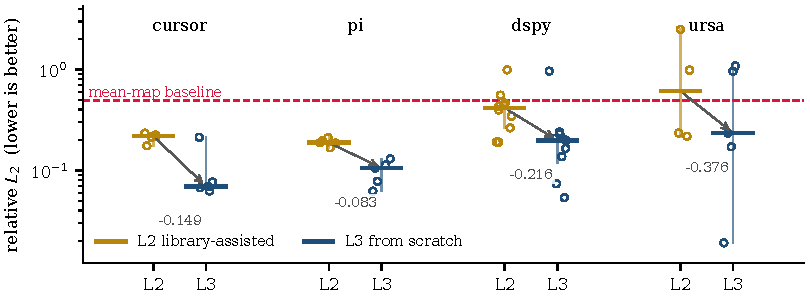
\includegraphics[width=0.92\textwidth]{figures/fig_levels}
\caption{Every scored run, by cell. Circles are individual replicates, the
heavy bar is the cell median with its bootstrap interval, and the arrow is the
within-harness \Ltwo{}$\rightarrow$\Lthree{} contrast, annotated with the
difference in medians. From-scratch is better in all four substrates. The two
substrates with the widest replicate spread are also the two that produce runs
worse than predicting the mean field.}
\label{fig:levels}
\end{figure}

Pooled across substrates, \Ltwo{} has median \relltwo{} $0.2287$ (bootstrap
$[0.211, 0.396]$, 24 scored runs) against \Lthree{}'s $0.1368$
($[0.077, 0.207]$, 25 runs). Contract pass rates are $24/33$ (Wilson
$[0.56, 0.85]$) and $25/26$ ($[0.81, 0.99]$). Accuracy per hundred solver calls
--- a crude efficiency measure, but one that accounts for agents that bought
their way to a better score --- is $10.31$ against $19.55$.

The paired differences are $-0.149$, $-0.216$, $-0.083$ and $-0.376$ for
\hn{cursor}, \hn{dspy}, \hn{pi} and \hn{ursa} respectively:
four substrates, four times in the same direction (Figure~\ref{fig:levels}).

Our primary test treats the harness as a blocking factor and permutes level
labels only within it --- a stratified rank statistic in the van Elteren
family~\citep{vanelteren1960combination}. It gives $z = -4.168$ with permutation
$p = 1/20\,001 \approx 5\times10^{-5}$. That $p$ is the resolution floor of the
test rather than a point estimate: zero of 20\,000 within-harness relabelings
reached the observed statistic. Substrate differences cannot inflate it,
because no permutation ever moves a run between harnesses.

Two other tests, reported because they differ in power rather than in
direction. The exact sign test on the four paired medians gives $0/4$ and
$p = 0.125$ --- the smallest two-sided $p$ attainable at four pairs, whatever
the data show. The originally pre-specified median-difference permutation test
gives $\delta = -0.206$, $p = 0.179$; it compresses each cell to a single
number and then has four numbers to work with. As set out in
Section~\ref{sec:analysis}, the switch of primary test was made after seeing
that a unanimous result could not clear the sign test's floor, and is post-hoc.

Two readings survive this. Library access might genuinely handicap an agent, or
the \Ltwo{} prompt's pointers into the library might anchor agents onto its
defaults. Section~\ref{sec:agentlogic} shows the anchoring is real and
measurable, and Section~\ref{sec:vs-baseline} bounds how much of the gap the
library's own quality could explain.

\subsection{Does the harness matter, with the model held fixed?}
\label{sec:harness-effect}

Yes --- and more than the access level does. With one model across all eight
cells, the per-cell medians span $0.0692$ to $0.6101$, a factor of $8.8$,
against the $1.7\times$ pooled level effect. Ordering the substrates by
\Lthree{} median gives \hn{cursor}, \hn{pi}, \hn{dspy}, \hn{ursa}; the same
order holds at \Ltwo{} but for \hn{pi} and \hn{cursor} swapping places.

The spread is not only in the median, and this is the part we did not expect.
\hn{cursor} and \hn{pi} produced twenty scored runs between them with
\emph{zero} physically invalid artifacts and a worst case of $0.234$. \hn{dspy}
and \hn{ursa} account for all fifteen invalid artifacts and every run that
scored worse than predicting the mean field. Same model, same task text, same
budget; the difference is the software wrapped around the model.

This is the comparison the literature usually confounds, and it is the
empirical form of a claim recently argued on other grounds --- that the harness,
not the model it wraps, is often the binding
constraint~\citep{zhang2026harness}.

\subsection{Against a baseline that uses no model at all}
\label{sec:vs-baseline}

The pre-written pipeline, run at \Lzero{} with seeded heuristic decisions and no
language model anywhere in the loop, scores mean \relltwo{} $0.1774$, $0.1865$
and $0.1863$ on three seeds at a budget matched to the agents' 450 successful
solves. That is about 63\% accuracy, in 83--101 seconds, for \$0.00 of model
spend. Given five times the data it reaches $0.1666$, so its budget is not what
limits it.

Against that line, \textbf{two of the eight agent cells beat the zero-model
baseline} --- \Lthree{}-\hn{cursor} and \Lthree{}-\hn{pi} --- one roughly
matches it, and five are worse. Both that beat it are from-scratch.

This constrains how Section~\ref{sec:l2l3} may be read. The library is not
simply bad code dragging \Ltwo{} down: it outperforms five of the eight agent
cells on the same frozen set. Whatever is happening at \Ltwo{} is better
explained by what library access does to the agent's search over methods than by
the quality of the library itself.

\subsection{Cost, and whether the budget was respected}
\label{sec:cost}

\begin{figure}[t]
\centering
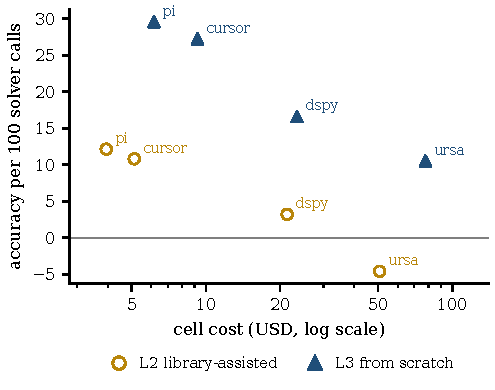
\includegraphics[width=0.56\textwidth]{figures/fig_cost}
\caption{What each cell's accuracy cost, at one model. A $13\times$ spread in
dollars buys no consistent advantage: the two cheapest substrates occupy the two
best positions, and the most expensive cell in the campaign sits below
\Lthree{}-\hn{pi} at one-thirteenth the price.}
\label{fig:cost}
\end{figure}

Cost is dominated by a single substrate. \hn{ursa} spent \$128.51 across 14
runs --- 65\% of the entire campaign --- against \$44.82 for \hn{dspy} (25
runs), \$14.36 for \hn{cursor} and \$10.10 for \hn{pi} (10 runs each). It buys
nothing legible (Figure~\ref{fig:cost}).

Costs are measured directly where a substrate reports dollars and otherwise
derived from token counts at a committed, dated price table. The \hn{cursor}
figure is an estimate at provider rates rather than that vendor's actual
billing, because that agent consumes its own product's quota; it is labelled
derived everywhere it appears.

On the 450-solve campaign bound, the median cell is compliant once the uncapped
validation and test solves are allowed for (medians of 239--689 attempted
solves). The exceptions are concentrated in \Ltwo{}-\hn{dspy}, whose worst runs
attempted 1914 and 1650 solves --- overruns of $+1464$ and $+1200$ against a
bound stated plainly in the prompt they were given. We report the raw
distribution rather than a pass/fail, since validation and test solves are
legitimately additional, but an overrun of four times the campaign budget is not
an accounting subtlety.

Wall-clock time is contaminated by running several cells concurrently on one
CPU-bound machine, and is not a reportable efficiency metric here. For
completeness, the campaign consumed 19.1 hours summed over 59 runs.
